\section{Generic Spaceship Architecture}
One of the most important characteristics of this domain is that spacecraft
missions have extremely diverse purpose, so the design of each is specific and
unique. The spacecrafts that go outside Earth's atmosphere vary from simple ones
(e.g. satellites) to very complicated ones (e.g. deep-space missions). However,
the principles on which their designs are based are common. Virtually all the
spacecrafts have similar requirements regarding aspects such as power,
telecommunications, propulsion etc. and share a general structural construction.
Thus, in order to aid the understanding of the Fault-Tolerant approaches used
for space missions, a generic architecture for spacecrafts is briefly described.

Typically, spaceships have an architecture that contains, at minimum, 6
subsystems\cite{ft-space-avionics}. These are \textit{propulsion},
\textit{communications}, \textit{power}, \textit{attitude control},
\textit{thermal control} and \textit{command \& control}, as seen in
Figure~\ref{fig:generic_structure}.

\begin{description}
  \item[Propulsion] This subsystem is in charge of accelerating and stabilizing
  the ship and controlling its orientation. Multiple methods can be used for
  propulsion, but the most common ones are gas\footnote{Chemical or pressurized
  gas is forced at a high speed through a nozzle. This is still the most common
  method.} or electric\footnote{Commonly ion thrusters or Hall effect thrusters
  are used.} based.
  \item[Communication] This subsystem handles the communication between the
  spaceship and the Earth control center. The spacecraft employs transmitters
  and receivers to send and receive messages which travel through space as radio
  waves. The communication going from a satellite to ground is called downlink
  and the one going from ground to a satellite is called uplink. Unlike the
  other modules, the Communications subsystem interfaces not only with
  components on the ship, but also with external entities.
  \item[Power] All the components of a spacrafts Spacecraft require electrical
  power for powering the various functions. This subsytem is in charge of the
  generation, storage and distribution of electrical energy in the spaceship.
  Various generation methods are employed\footnote{ For ships near the Sun,
  solar panels are frequently used to generate electrical power. In more distant
  locations, for example Jupiter, might employ a Radioisotope Thermoelectric
  Generator (RTG) to generate electrical power.}, the most common one involving
  solar cells. The power is passed through a power distribution unit over an
  electrical bus to other spacecraft components. Batteries are used to provide
  electrical power during periods when primary power is not available.
  \item[Attitude Control] This subsystem handles the correct orientation and
  stability of the spacecraft by computing the response to external torques and
  forces. Its main components are sensors and actuators and uses specialized
  algorithms for control.
  \item[Thermal Control] As temperatures in the surrounding environment may vary
  by hundreds of degrees, the ships require this subsystem to assure that all
  the components have a proper temperature. It can be passive, such as
  insulations, special materials etc., or active, employing electrical heaters
  to manipulate the temperature of the components.
  \item[Command/Control] All the aspects related to the spaceship's control are
  handled by this subsystem. Its main tasks include: receives commands from
  the communications subsystem; validates, decodes and distributes the commands
  to the appropriate spacecraft components; receives internal and scientific
  data from the other spacecraft subsystems and components and packages the data
  for storage on a data recorder or transmission to the ground. Also, this
  subsystem is in charge of system health-monitoring and recovery from failures.
\end{description}

Besides these main components, most of the deep space exploration ships have a
\textbf{payload of scientific instruments} (usually simply refered to
as \textit{payload}), that are used to gather various types of data from the
surrounding environment. A few examples of scientific instruments used are
magnetometers, energetic particle detectors, temperature sensors,
spectrometers, radiation sensors, high resolution cameras.

\begin{figure}[htb]
	\begin{center}
	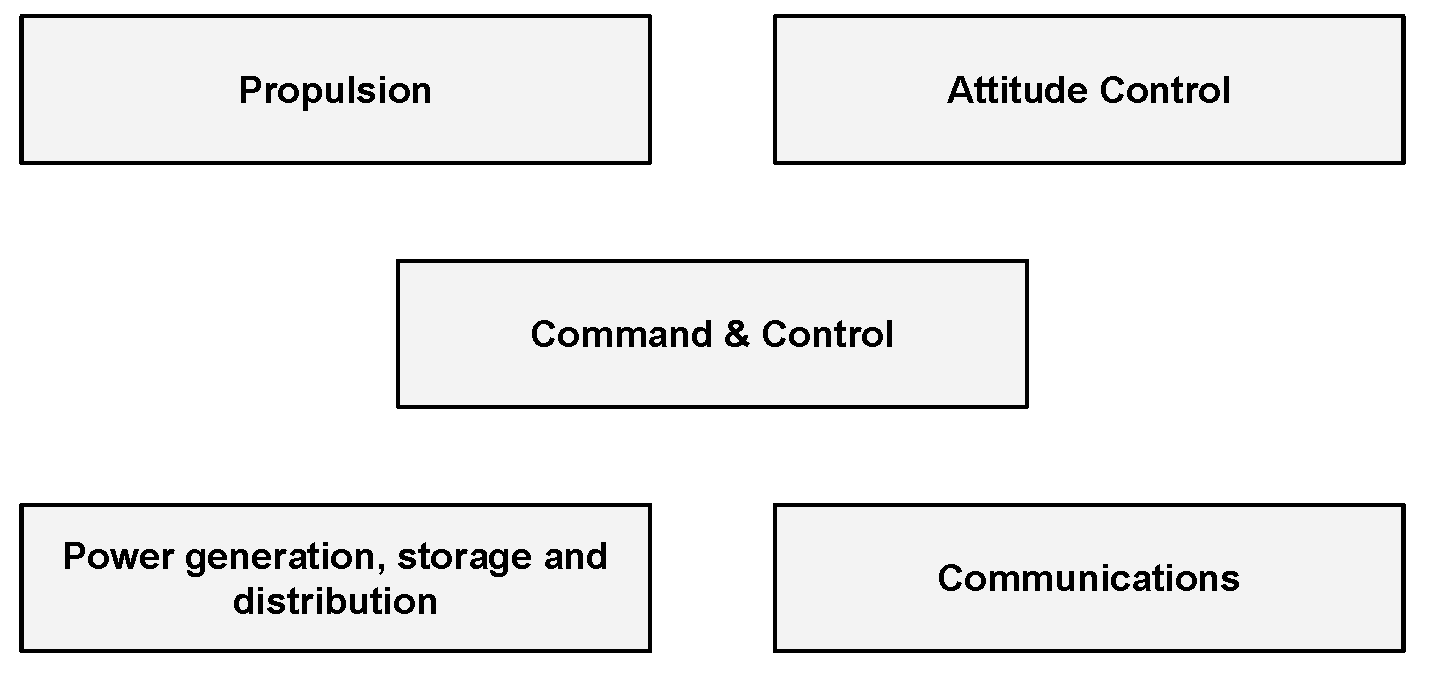
\includegraphics[width=0.92\textwidth]{img/generic_structure.pdf}
	\caption{Components of Generic Spacecraft}
	\label{fig:generic_structure}
	\end{center}
\end{figure}
\todo{Add missing 2 components}